% Template from Usenix
\documentclass[letterpaper,twocolumn,10pt]{article}
\usepackage{usenix,epsfig,endnotes}
\usepackage{graphicx}

\begin{document}

% Don't output date
\date{}

% Title
\title{\Large \textbf{
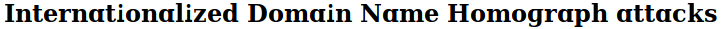
\includegraphics[height=\baselineskip]{title} \\
Project Proposal } \\ \vspace{0.025 in} \large \normalfont
CSE 227: Computer Security - Spring 2017 \\ \textit{
University of California San Diego
}}

% Authors
\author{
{\rm Chen Lai}\\
\normalfont{\texttt{chl588@ucsd.edu}}
\and
{\rm Zhongrong Jian}\\
\normalfont{\texttt{zhjian@ucsd.edu}}
\and
{\rm Juan Sidrach}\\
\normalfont{\texttt{jsidrach@ucsd.edu}}
}

\maketitle

\section{What}
- Explain the attack
  - When/how were IDN introduced
  - Homograph letters
  - How to use this to the attackers advantage

- Research
  - On websites
    - Top 500 Alexa Websites
    - Try all possible variations
    - Classify: 404, redirect (legitimate), malicious, unrelated
    - Evaluation
  - On browsers
    - % Affected, version affected
    - Screenshots before/after CVE (url bar, hover link)
    - Other possible policies: why they may work or they won't
      - Maybe domain providers should not allow IDNs close to real names?
      - Whitelist/blacklist

- Conclusion
  - Impact of the vulnerability based on empirical data and % of users still vulnerable

\section{Why}
- Relatively new CVE discovered because this (https://bugs.chromium.org/p/chromium/issues/detail?id=683314)
- How something beneficial for the users IDN could be turned against them
- Hard for regular users to distinguish between real/fake sites
- Easy to collect data to evaluate impact

\section{Potential Issues}
- The potential impact, it may be actually really low
- If we will find not legitimate sites by substitution (sample size may be low)
- If there are a lot of illegitime sites, we would need to check manually if they are just a redirect or a scam, maybe we will need to find an automatic way

\section{Resources}
Resources
- We believe for the TOP500 sites + variations of each one we can check it with our own computers/crawlers, same for different browsers


\end{document}
